\documentclass{beamer}
\usepackage[polish]{babel}
\usepackage[utf8]{inputenc}
\usepackage{lmodern}
\usepackage{polski}
\usepackage{amsfonts}
\usepackage{eufrak}
\usepackage{indentfirst}
\usepackage{amsthm}
\usepackage{multirow}
\usepackage{amsmath}
\usepackage{graphicx}
\newcommand{\norm}[1]{\left\lVert#1\right\rVert}
\usetheme{AGH}

\title{Stochastyczne problemy odwrotne}
\subtitle{Definicje i zastosowania}
\author{Grzegorz Mika}
\institute{Wydział Matematyki Stosowanej}

\date{9 czerwca 2018}

\begin{document}

\titleframe[pl]


\begin{frame}\frametitle{Początki}
	\begin{center}
		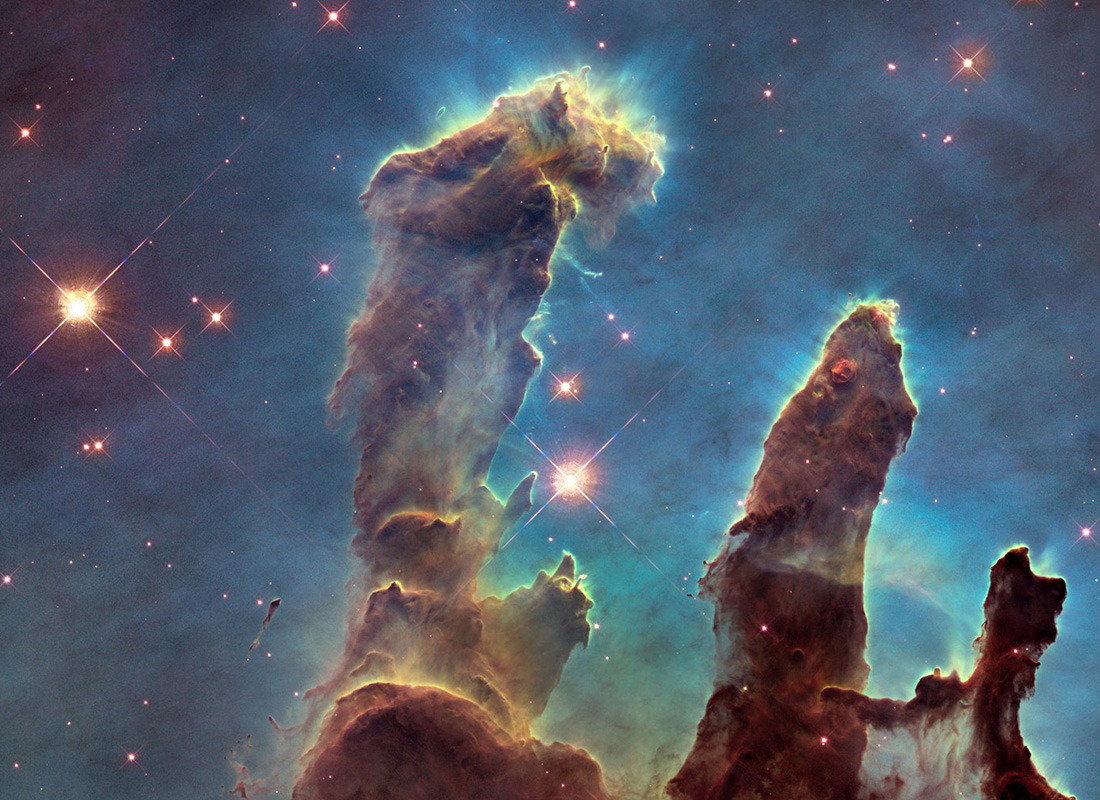
\includegraphics[scale=0.132]{4}
		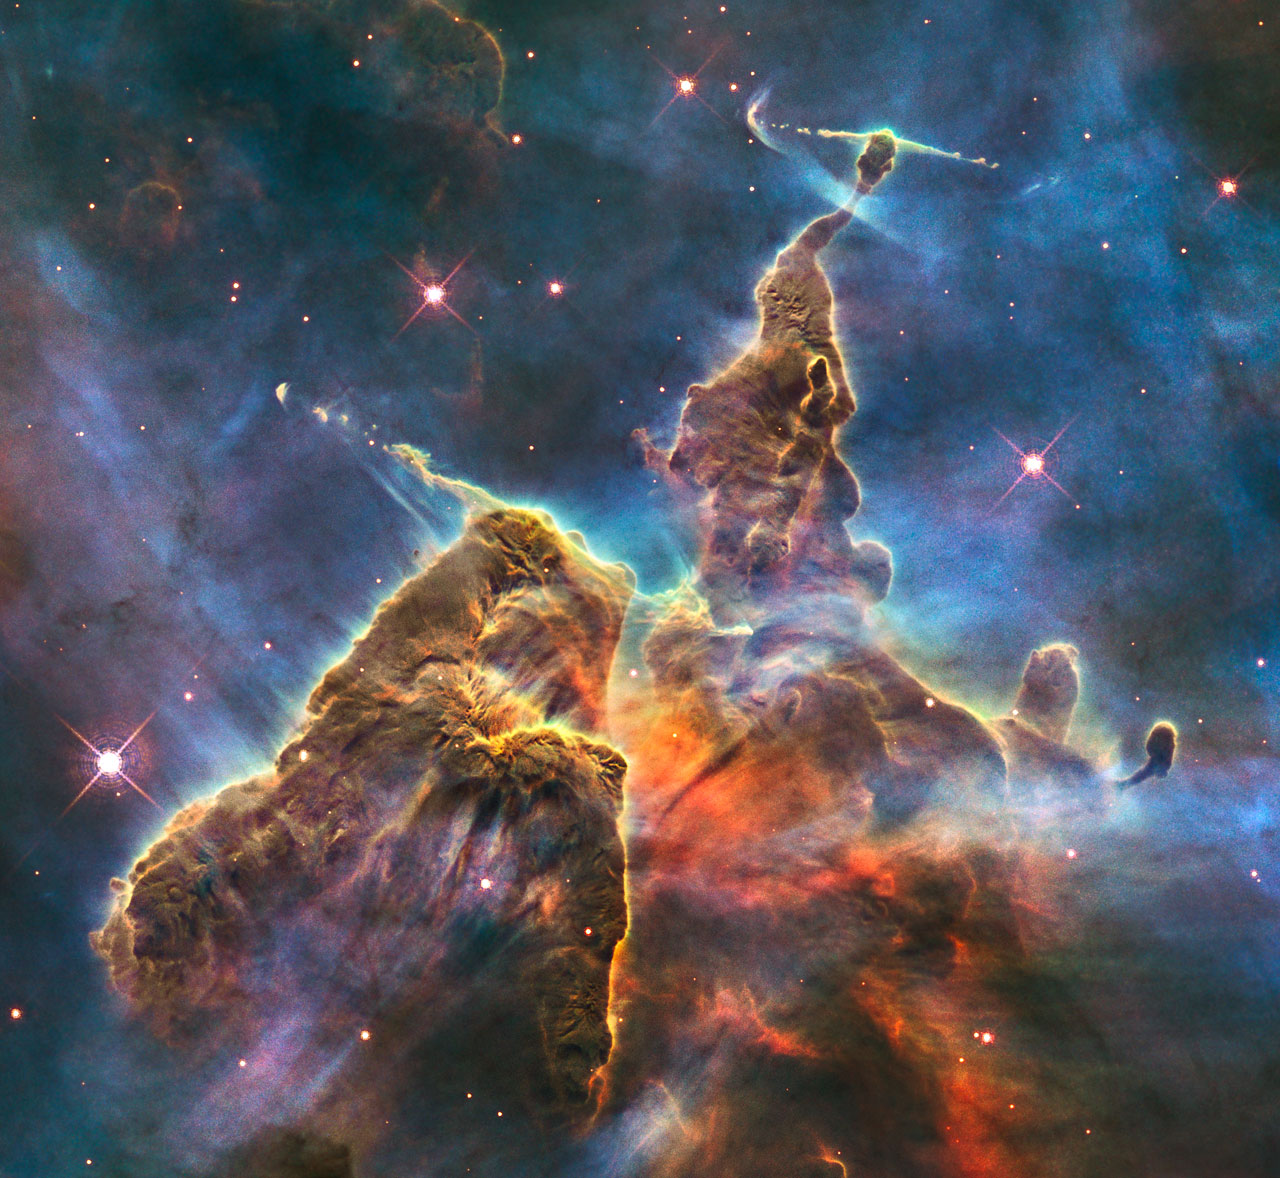
\includegraphics[scale=0.09]{3}
	\end{center}
	\begin{center}
		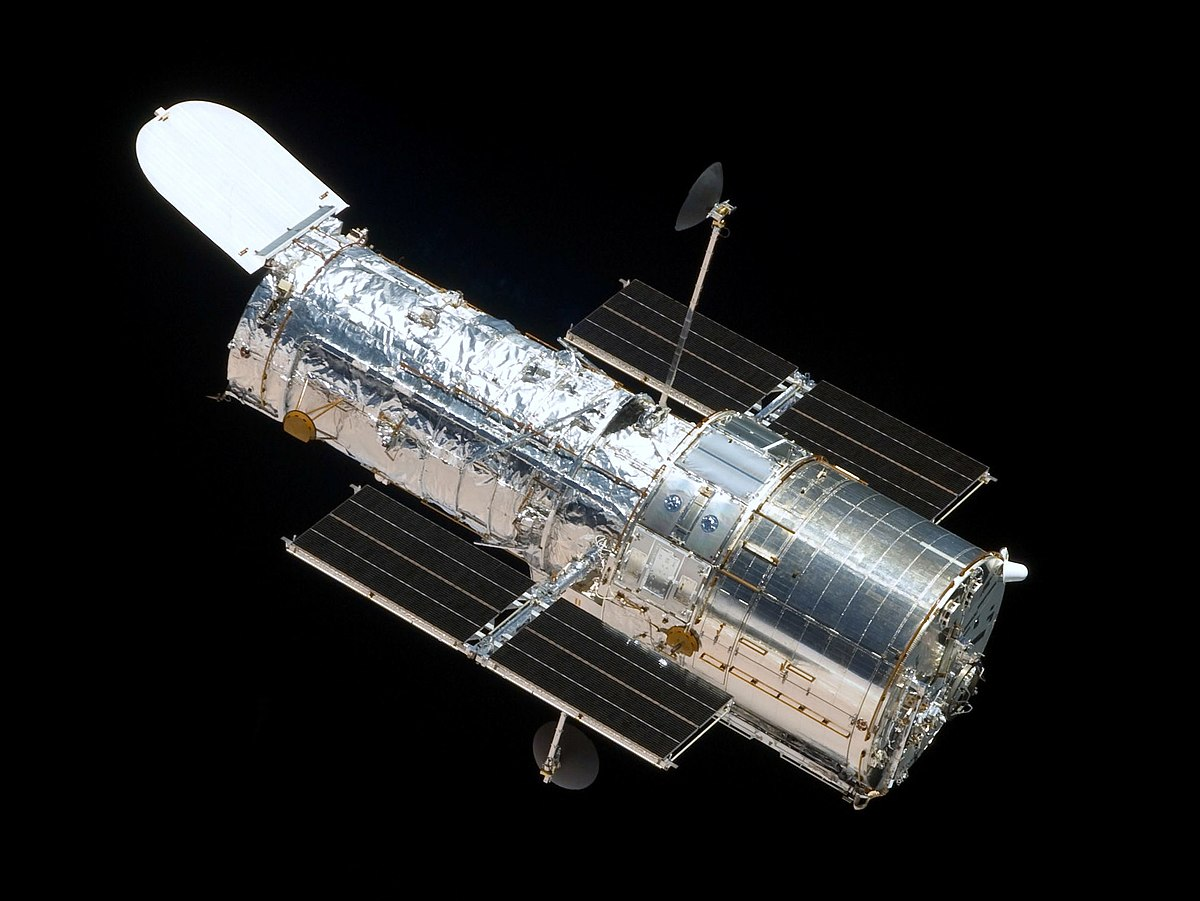
\includegraphics[scale=0.09]{2}
	\end{center}
\end{frame}

\begin{frame}\frametitle{Początki}
\begin{center}

\includegraphics[scale=0.4]{6}
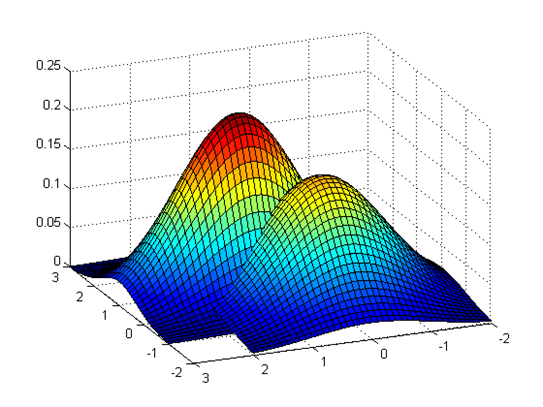
\includegraphics[scale=0.4]{5}
\end{center}
\end{frame}

\begin{frame}\frametitle{Początki}\framesubtitle{Matematyczny opis}

\begin{block}{Stochastyczny problem odwrotny}
\begin{displaymath}
Y=Kf+\epsilon\xi
\end{displaymath}
\begin{displaymath}
K\colon \mathbb{H}\to \mathbb{G}, \epsilon>0
\end{displaymath}
\end{block}
\begin{block}{Hubble}
\begin{displaymath}
Y=\int_Dh(\cdot-x)f(x)dx+\epsilon\xi
\end{displaymath}
\begin{displaymath}
\mathbb{H}= \mathbb{G}=L_2(\mathbb{R}^2), h\colon \mathbb{R}^2\to \mathbb{R}
\end{displaymath}
\end{block}
\end{frame}

\begin{frame}\frametitle{Naiwne podejście}
\begin{block}{Stochastyczny problem odwrotny}
\begin{displaymath}
Y=Kf+\epsilon\xi
\end{displaymath}
\begin{displaymath}
K\colon \mathbb{H}\to \mathbb{G}, \epsilon>0
\end{displaymath}
\end{block}
\end{frame}

\begin{frame}\frametitle{Naiwne podejście}
\begin{block}{Stochastyczny problem odwrotny}
\begin{displaymath}
Y=Kf+\epsilon\xi
\end{displaymath}
\begin{displaymath}
K\colon \mathbb{H}\to \mathbb{G}, \epsilon>0
\end{displaymath}
\end{block}
\begin{block}{}
\begin{itemize}
\item skonstruować estymator $\hat{g}$ dla $g=Kf$ na bazie obserwacji $Y$
\end{itemize}
\end{block}
\end{frame}

\begin{frame}\frametitle{Naiwne podejście}
\begin{block}{Stochastyczny problem odwrotny}
\begin{displaymath}
Y=Kf+\epsilon\xi
\end{displaymath}
\begin{displaymath}
K\colon \mathbb{H}\to \mathbb{G}, \epsilon>0
\end{displaymath}
\end{block}
\begin{block}{}
\begin{itemize}
\item skonstruować estymator $\hat{g}$ dla $g=Kf$ na bazie obserwacji $Y$,
\item estymować $f$ przez $K^{-1}\hat{g}$.
\end{itemize}
\end{block}
\end{frame}

\begin{frame}\frametitle{Naiwne podejście}
\begin{center}
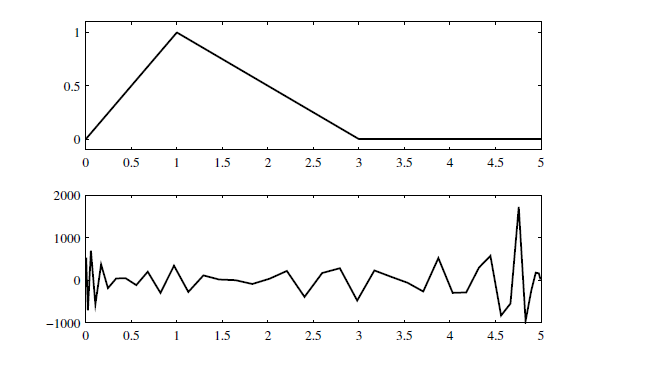
\includegraphics[scale=0.65]{7}
\end{center}
\end{frame}

\begin{frame}\frametitle{Uwarunkowanie problemu}
\begin{block}{Uwarunkowanie problemu}
Problem nazwiemy dobrze postawionym w sensie Hadamarda, gdy:
\begin{itemize}
\item dla dowolnego $g\in \mathbb{G}$ istnieje $f\in \mathbb{H}$ spełniający zadane równanie,
\item rozwiązanie jest jedyne,
\item rozwiązanie jest stabilne, czyli zależy w sposób ciągły od prawej strony równania.
\end{itemize}
\end{block}
\end{frame}

\begin{frame}\frametitle{Uwarunkowanie problemu}
\begin{block}{Uwarunkowanie problemu}
Problem $Kf=g$ nazwiemy dobrze postawionym w sensie Hadamarda, gdy:
\begin{itemize}
\item dla dowolnego $g\in \mathbb{G}$ istnieje $f\in \mathbb{H}$ spełniający zadane równanie,
\item rozwiązanie jest jedyne,
\item rozwiązanie jest stabilne, czyli zależy w sposób ciągły od prawej strony równania.
\end{itemize}
\end{block}
\begin{block}{Problem}
Większość ''naturalnie występujących'' problemów jest źle uwarunkowana!
\end{block}
\end{frame}


\begin{frame}\frametitle{Regularyzacja}
\begin{block}{}
Rozwiązaniem w sensie średniokwadratowym nazywamy $f^*$ takie, że
\begin{displaymath}
\norm{Af^*-g}=\inf\left\{\norm{Au-g},u\in \mathbb{H}\right\}.
\end{displaymath}
\end{block}
\begin{block}{Prekondycjonowanie}
$f^*$ jest rozwiązaniem w sensie średniokwadratowym wtedy i tylko wtedy, gdy
\begin{displaymath}
A^*Y=A^*Af+\epsilon A^*\xi,
\end{displaymath}
gdzie $A^*$ jest sprzężeniem operatora $A$.
\end{block}
\end{frame}

\begin{frame}\frametitle{Regularyzacja}
\begin{block}{"Delikatne'' odwrócenie}
\begin{displaymath}
\hat{f}_{\alpha}=\Phi_{\alpha}(A^*A)A^*Y,
\end{displaymath}
\end{block}
\begin{block}{}
\begin{displaymath}
\sup_{t\geq 0}\Phi_{\alpha}(t)<\infty\ \forall \alpha>0
\end{displaymath}
\begin{displaymath}
\sup_{\alpha>0,t\geq 0}t\Phi_{\alpha}(t)<\infty
\end{displaymath}
\begin{displaymath}
\Phi_{\alpha}(t)\to t^{-1},\ gdy\  \alpha\to 0,\ \forall t>0
\end{displaymath}
\end{block}
\end{frame}

\begin{frame}\frametitle{Przyjazna postać}
\begin{block}{Twierdzenie spektralne w wersji Halomsa}
Niech $A$ będzie operatorem samosprzężonym na ośrodkowej przestrzeni Hilberta $H$. Wtedy istnieje przestrzeń mierzalna $(S,\mathcal{S},\mu )$, rzeczywista funkcja mierzalna $b$ określona na $S$ i operator unitarny $U\colon H\to L_2(S,\mathcal{S},\mu )$, takie, że 
\begin{displaymath}
A=U^{-1}M_bU,
\end{displaymath}
gdzie $M_b$ jest operatorem mnożenia przez funkcję $b$ zdefiniowanym jako $(M_bg)(x)=b(x)g(x)$.
\end{block}
\begin{block}{}
\begin{center}
W źle uwarunkowanych problemach $b\to 0$.
\end{center}
\end{block}
\end{frame}

\begin{frame}\frametitle{Przyjazna postać}
\begin{block}{}
Problem
\begin{displaymath}
A^*Y=A^*Af+\epsilon A^*\xi
\end{displaymath}
ma przedstawienie
\begin{displaymath}
UA^*Y=b\theta+\epsilon\eta
\end{displaymath}
lub równoważnie
\begin{displaymath}
X=\theta+\epsilon\sigma\eta
\end{displaymath}
\end{block}
\begin{center}
$\sigma=\frac{1}{b}$, $\theta=Uf$, $\eta=UA^*\xi$.
\end{center}
\end{frame}

\begin{frame}\frametitle{Czy to ma sens?}
\begin{block}{Najprostsza regularyzacja}
\begin{displaymath}
\Phi_{\alpha}(t)=\frac{1}{t}\pmb{1}_{[\alpha,\infty)}
\end{displaymath}
\end{block}
\end{frame}



\begin{frame}\frametitle{Czy to ma sens?}
\begin{block}{Najprostsza regularyzacja}
\begin{displaymath}
\Phi_{\alpha}(t)=\frac{1}{t}\pmb{1}_{[\alpha,\infty)}
\end{displaymath}
\end{block}
\begin{center}
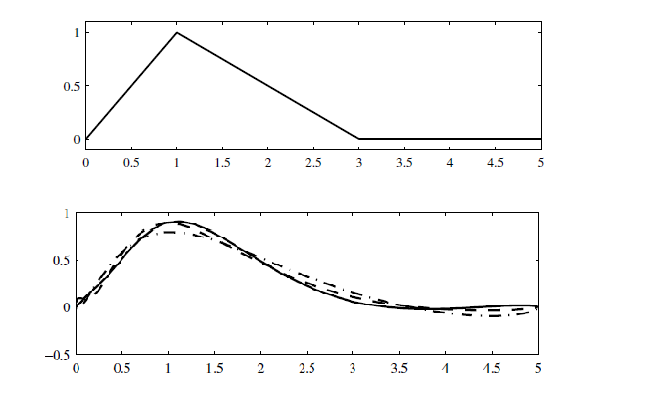
\includegraphics[scale=0.45]{8}
\end{center}
\end{frame}

\begin{frame}\frametitle{Zastosowania}
\begin{center}
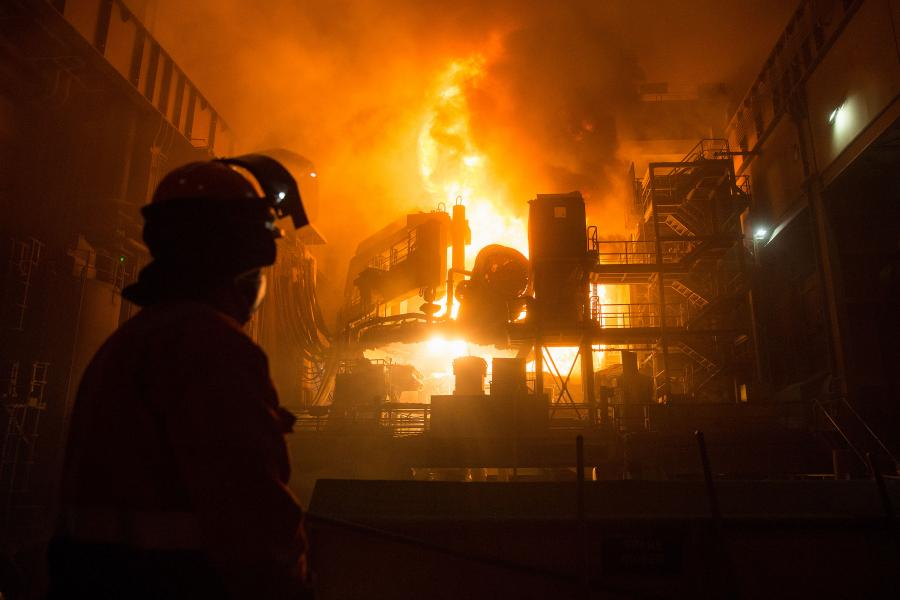
\includegraphics[scale=0.145]{a}
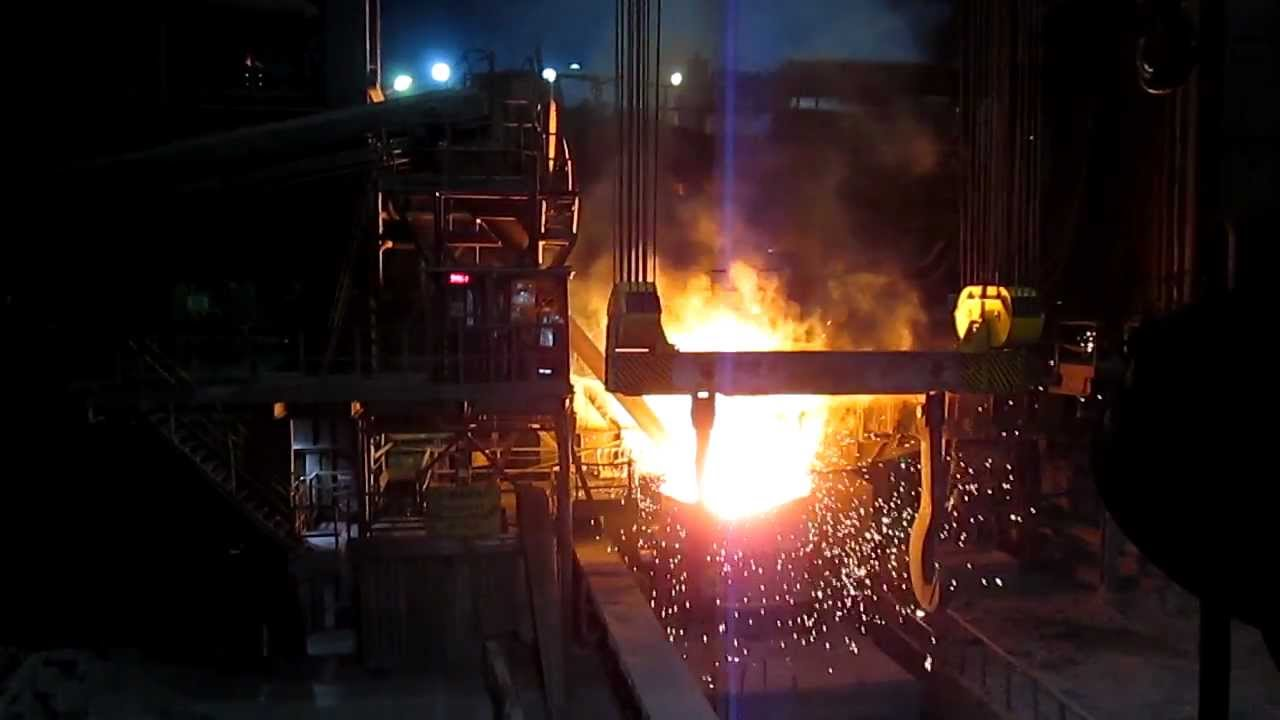
\includegraphics[scale=0.12]{b}
\end{center}
\begin{center}
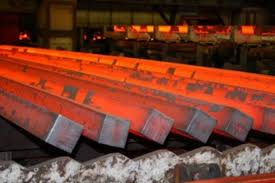
\includegraphics[scale=0.5]{c}
\end{center}
\end{frame}

\begin{frame}\frametitle{Zastosowania}
\begin{center}
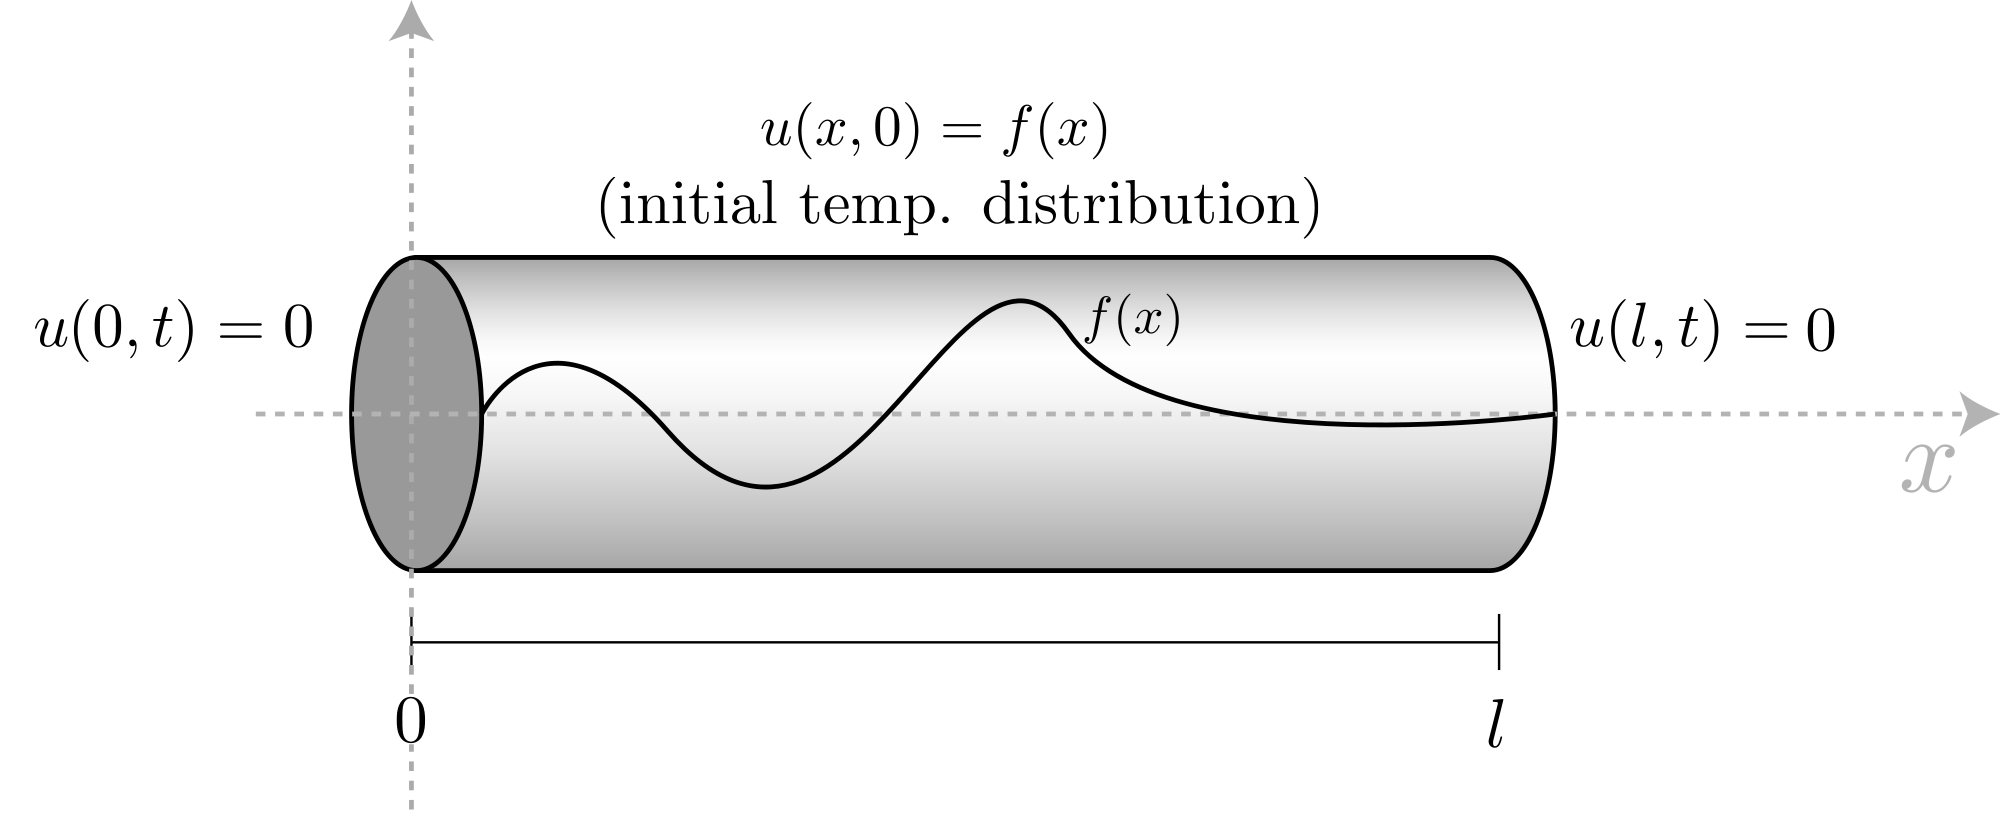
\includegraphics[scale=0.1]{9}
\end{center}
\begin{block}{Równanie ciepła}
\begin{displaymath}
\frac{\partial}{\partial t}u(x,t)=\frac{\partial^2}{\partial x^2}u(x,t),\ u(x,0)=f(x),\ u(0,t)=u(1,t)=0
\end{displaymath}
\begin{displaymath}
Af=\int_0^1\sum_{k=1}^{\infty}2\exp (-\pi^2k^2T)\sin (k\pi x)\sin (k\pi y)f(y)dy
\end{displaymath}
\end{block}
\end{frame}

\begin{frame}\frametitle{Zastosowania}
\begin{center}

\includegraphics[scale=0.5]{d}

\includegraphics[scale=0.3]{e}
\end{center}
\begin{center}

\includegraphics[scale=0.5]{f}
\end{center}
\end{frame}

\begin{frame}\frametitle{Zastosowania}
\begin{block}{Zmienne ukryte}
\begin{displaymath}
(\tilde{y},z,w)\sim F
\end{displaymath}
\begin{displaymath}
\left\{{\tilde{y}=x_0(z)+U}\atop {\mathbb{E}(U|w)=0}\right.
\end{displaymath}
\begin{displaymath}
A\colon x\to \mathbb{E}(x(z)|w),\ y=\mathbb{E}(\tilde{y}|w)
\end{displaymath}
\begin{displaymath}
y=\hat{A}x_0+\left[Ax_0-\hat{A}x_0\right]=\hat{A}x_0+\epsilon\xi
\end{displaymath}
\end{block}
\end{frame}




\begin{frame}\frametitle{Bibligrafia}
\begin{thebibliography}{100}
\bibitem{forsal} Strona \emph{forsal.pl},
\bibitem{Phd} Strona \emph{phdcomics.com},
\bibitem{crazy} Strona \emph{crazynauka.pl},
\bibitem{love} Strona \emph{nauklove.pl},
\bibitem{rev} J.- M. Loubes, V. Rivoirard, \emph{Review of rates pf convergance and reularity conditions for inverse problems}, technical report,
\bibitem{kaipo}
J. Kaipio, E. Somersalo, \emph{Statistical and Computational Inverse Problems}, Springer, 2004,
\bibitem{iphde} P. Alquier,	E. Gautier, G. Stoltz, \emph{Inverse Problems and High-Dimensional Estimation}	Springer-Verlag, 2011, wydanie zbiorowe,
\end{thebibliography}
\end{frame}

\begin{frame}\frametitle{Koniec}
\begin{center}
\huge{\textbf{Dziękuję za uwagę!}}
\end{center}
\end{frame}
\begin{frame}\frametitle{Rezultaty}
\begin{center}

\includegraphics[scale=0.16]{1}
\end{center}
\end{frame}
\end{document}
